%%%%%%%%%%%%%%%%%%%%%%%%%%%%%%%%%%%%%%%%%%%%%%%%%%%%%%%%%%%%%%%%%
%
% Project     : Bachelorarbeit
% Title       : Machbarkeitsanalyse für eine ressourcenorientierte Schnittstelle zur Verarbeitung grundlegender Probleme der Informatik
% File        : tests.tex Rev. 01
% Date        : 01.03.2015
% Author      : Raffael Santschi
%
%%%%%%%%%%%%%%%%%%%%%%%%%%%%%%%%%%%%%%%%%%%%%%%%%%%%%%%%%%%%%%%%%

\chapter{Tests \resultAssignment{[R6]}}\label{chap.tests} 
In diesem Kapitel wird auf das Testverfahren und die Tests für den Prototyp eingegangen.

\section{Einführung}
In diesem Projekt wurden die sieben Grundsätze aus \cite{test_soft_book} als Leitlinie zum Testen verwendet:
\begin{enumerate}
\item \textbf{Testen zeigt die Anwesenheit von Fehlern}: Die Testabdeckung wurde mit Hilfe von IntelliJ ermittelt und anhand des Testsprotokolls überprüft, ob alle Bereiche abgedeckt wurden.
\item \textbf{Vollständiges Testen ist nicht möglich}: Es wurde solange getestet bis alle Akzeptanzkriterien abgedeckt waren und die Testabdeckung gut genug war.
\item \textbf{Mit dem Testen frühzeitig beginnen}: Die Unit Tests für neue Funktionen wurden möglichst zeitnah oder zur gleichen Zeit geschrieben.
\item \textbf{Häufung von Fehlern}: Wenn Fehler in einer Komponente auftraten, dann wurde diese nach der Behebung nochmals intensiv getestet und zusätzliche Tests erfasst.
\item \textbf{Zunehmende Testresistenz (Pesticide paradox)}: Jede Änderungen am Code hatte auch eine Anpassung oder Erweiterung der Tests zur Folge.
\item \textbf{Testen ist abhängig vom Umfeld}: Der Prototyp ist nicht sicherheitskritisch, jedoch wurde Wert auf eine hohe Testabdeckung gelegt. Es wurden zusätzlich immer wieder 
	End-zu-End Tests mit den verschiedenen Problemen durchgeführt.
\item \textbf{Trugschluss: Keine Fehler bedeutet ein brauchbares System}: Die Schnittstelle wurde dem \gls{stakeholder} demonstriert und erklärt bevor das Projekt zu Ende war. So 
	konnten allfällige Missverständnise frühzeitig erkannt werden. Die hohe Testabdeckung trägt ebenfalls zur Aufdeckung von unbemerkten Fehlern bei.
\end{enumerate}

\section{Testing}
Komponententests und Integrationstests, bekannt aus \cite{test_soft_book}, wurden bei der Schnittstelle mit JUnit und Mockito durchgeführt. Bei den Integrationstests wurde eine 
Testdatenbank verwendet, welche bei jedem Testlauf neu initialisiert wird. Die Ausgangslage ist somit für jeden Durchlauf identisch. Für die Analyse der Testabdeckung wurde IntelliJ 
verwendet und die statische Code Analyse wurde mit \gls{sonar} ausgeführt. Neben den automatischen Tests wurden immer wieder manuelle Tests durchgeführt, um auch das Nutzererlebnis 
zu testen.

\subsection{Testabdeckung}
Es konnte nahezu eine 90\% Testabdeckung über das ganze Projekt erreicht werden (siehe \autoref{fig:test_coverage}). Unter den nicht getesteten Klassen und Methoden sind 
Konfigurationsdateien und private Konstruktoren, welche nicht bzw. nur schwierig zu testen sind. Bei den Tests konnte ebenfalls von dem generischen Aufbau profitiert werden, sodass die 
Controller und Services mit sehr wenig spezifischem Code getestet werden konnten.

\begin{figure}[h]
\centering
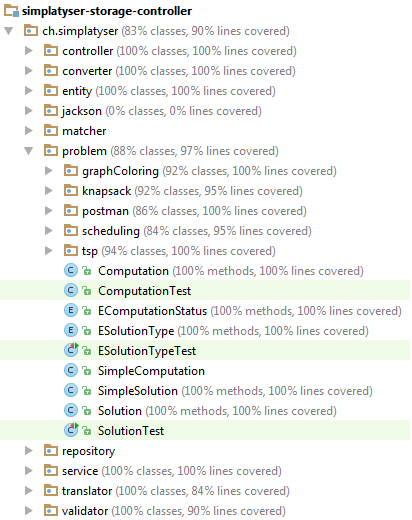
\includegraphics[scale=0.74]{images/test_coverage.png}
\caption[Analyse der Testabdeckung des Projekts]{Analyse der Testabdeckung des Projekts \selfmade{}}
\label{fig:test_coverage}
\end{figure}

\section{Systemtest}
Als Abschluss des Projekts wurde ein Systemtest durchgeführt, für welcher ein Testprotokoll erstellt wurde. Das Protokoll zeigt dem Kunden die Testabfolge und das Ergebnis.

\subsection{Testprotokoll}
Das Testprotokoll basiert auf den Use Cases (siehe Abschnitt \ref{use_cases}) und den Anforderungen (Abschnitt \ref{anforderungen}). Akzeptanzkriterien mit UND- oder ODER-Verknüpfung 
wurden aufgesplittet, um sicher zu gehen, dass beide Bedingungen erfüllt sind.

%%\begin{longtable}{ l | p{7cm} | l | l }
\begin{longtable}{>{\raggedright}m{1cm}m{6cm}m{3.5cm}m{3cm}}

\caption[Testprotokoll]{\label{table:tests}Testprotokoll}\\ 
\toprule
\textbf{ID}&\textbf{Test}&\textbf{Herkunft}&\textbf{nicht / teilweise / erfüllt}\\ \midrule\addlinespace
\endfirsthead
\caption*{\textbf{Tabelle~\ref{table:tests} (Fortsetzung):} Testprotokoll}\\ \toprule
\textbf{ID}&\textbf{Test}&\textbf{Herkunft}&\textbf{nicht / teilweise / erfüllt}\\ \midrule\addlinespace
\endhead

\bottomrule\multicolumn{2}{>{\small\raggedleft\arraybackslash}r}{\slshape Fortsetzung auf der nächsten Seite}\\
\endfoot
\bottomrule
\endlastfoot	

	\addlinespace
	1	&	Der Nutzer kann eine Schnittstelle für die bereitgestellte Berechnungsfunktionen ansprechen.			
				&	\nameref{table:req_1} 	&	erfüllt\\ \addlinespace\hline \addlinespace
	2	&	Die Parameter sind persistent.			
				&	\nameref{table:req_3} 	&	erfüllt\\ \addlinespace\hline \addlinespace
	3a	&	Es gibt eine Fehlermeldung, falls bei der Speicherung etwas fehlschlägt			
				&	\nameref{table:req_3} 	&	erfüllt\\ \addlinespace\hline \addlinespace
	3b	&	oder die Eingabeparameter nicht gültig sind.			
				&	\nameref{table:req_3} 	&	erfüllt\\ \addlinespace\hline \addlinespace				
	4	&	Der Nutzer erhält nach dem Start einer Berechnung eine ID.
				&	\nameref{table:req_2} 	&	erfüllt\\ \addlinespace\hline \addlinespace
	5a	&	Der Befehl für den Start wird versendet		
				&	\nameref{table:req_4} 	&	erfüllt\\ \addlinespace\hline \addlinespace
	5b	&	und die ID dabei übergeben.		
				&	\nameref{table:req_4} 	&	erfüllt\\ \addlinespace\hline \addlinespace				
	6	&	Die Fehlermeldung bei einem Fehlversuch wird gespeichert.
				&	\nameref{table:req_4} 	&	erfüllt\\ \addlinespace\hline \addlinespace
	7	&	Das Verarbeitungssystem erhält die Eingabeparameter.
				&	\nameref{table:req_5} 	&	erfüllt\\ \addlinespace\hline \addlinespace
	8	&	Das Verarbeitungssystem erhält eine Fehlermeldung, falls keine Eingabeparameter vorhanden sind.
				&	\nameref{table:req_5} 	&	erfüllt\\ \addlinespace\hline \addlinespace
	9	&	Der Nutzer erhält einen Status seiner Berechnung.
				&	\nameref{table:req_6} 	&	erfüllt\\ \addlinespace\hline \addlinespace
	10	&	Der Nutzer wird über die Änderungen des Status auf dem eingetragen Dienst informiert.
				&	\nameref{table:req_7} 	&	erfüllt\\ \addlinespace\hline \addlinespace
	11	&	Das Verarbeitungssystem kann das Resultat abspeichern.
				&	\nameref{table:req_8} 	&	erfüllt\\ \addlinespace\hline \addlinespace
	12	&	Das Verarbeitungssystem erhält eine Fehlermeldung, falls das Speichern fehlgeschlagen ist.
				&	\nameref{table:req_8} 	&	erfüllt\\ \addlinespace\hline \addlinespace
	13	&	Der Nutzer erhält das Resultat der Berechnung.
				&	\nameref{table:req_9} 	&	erfüllt\\ \addlinespace\hline \addlinespace
	14	&	Der Nutzer erhält eine entsprechende Fehlermeldung, wenn beim Bereitstellen des Resultats ein Fehler aufgetreten ist.
				&	\nameref{table:req_9} 	&	erfüllt\\ \addlinespace\hline \addlinespace
	15	&	Das Interface kann verwendet werden, ohne dass das Verarbeitungssystem bekannt ist.
				&	\nameref{table:req_nf_1} 	&	erfüllt\\ \addlinespace\hline \addlinespace
	16	&	Unterschiedliche Ausprägungen eines Problems benutzen das gleiche API.
				&	\nameref{table:req_nf_2} 	&	teilweise erfüllt\\ \addlinespace\hline \addlinespace
	17	&	Unterschiedliche Probleme haben kein abweichendes Persistierungsschema.
				&	\nameref{table:req_nf_3} 	&	erfüllt\\ \addlinespace\hline \addlinespace
	18	&	Die Schnittstelle kann mit wenig Aufwand erweitert werden.
				&	\nameref{table:req_nf_4} 	&	erfüllt\\ \addlinespace\hline \addlinespace					

\end{longtable}